\chapter{Discussion and Future Work}
While we show that the \ac{wse} can be used effectively to accelerate two-dimensional stencil codes and how tiling across the x and y dimensions can be used to achieve higher throughput, more work is needed to further optimize the performance, extend the approach to other stencil patterns and automating code generation for the \ac{wse}.

\section{Performance and Kernel-Level Optimizations}
There are several possible ways to further optimize our proposed implementation.
First, implementing strict overlap between communication and computation would lead to increased utilization of the available compute resources and increase the throughput, especially for larger radii.
For the outermost row or column of the halo region, this could be easily implemented by multiplying the values while receiving directly with the specific coefficient and adding the results to the accumulator. In the computation step, the \acp{dsd} could be cropped to only include not yet computed values. However for the general case with a radius greater than one, multiple grid values depend on the same third grid value, making this problem highly complex. To take this idea one step further, computation can also be done while sending the data, but it is unclear whether it would be theoretically feasible to reorganize the compute in the necessary way.

Furthermore, we could not achieve full \ac{simd} width for the \texttt{@fadds} instruction, specifically measuring an average of 1.25 operations per cycle on \ac{wse}-2 and 1.5 operations per cycle on \ac{wse}-3. Even for \texttt{@fmacs} instructions that have a maximum \ac{simd} width of one, we could not achieve a sustained throughput of one operation per cycle. Full \ac{simd} width can only be reached if the two source operands reside in banks that do not conflict with each other. The bank number in which data lies only depends on the absolute memory address, so that bank conflicts can be avoided by having specific offsets between the addresses of operands. In the current implementation however, different regions within the buffer with offsets between 0 and $r$ in x and y direction relative to the center are added to the accumulator which has a fixed address.
This necessarily creates operations where bank conflicts occur.
A tile-size dependent padding could probably decrease the number of conflicts, but a more robust solution is possible.
By defining both the buffer and accumulator with an equal, carefully chosen memory pitch, conflicts can be eliminated altogether if a specific offset is maintained between the two data structures.
A naive implementation of this idea would be very memory-wasteful.
However, if the buffer and accumulator are defined as interleaved views using \acp{dsd} within the same physical memory block, the overhead can be significantly reduced by "sharing the sparsity."
In limited experiments we could not achieve  full \ac{simd} width using \texttt{mem4d\_dsd}s, even in settings with no bank conflicts. We are not sure whether this might have been caused by inherent limitations of \texttt{mem4d\_dsd}s or other factors.

We explored the potential of optimization by trading \texttt{@fmacs} instructions for \texttt{@fadds} and \texttt{@fmuls} instructions for problems with symmetric coefficients in the r1-optimized implementation. The logical next step would be to dynamically recognize if symmetric coefficients are used and switch to  this more computationally efficient kernel, which would reduce the cycles per cell from four to three on \ac{wse}-2 and two on \ac{wse}-3 respectively.

Overhead could be further reduced by strictly using explicit \ac{dsr} assignment, better utilization of border \acp{pe} and more efficient logic to detect the completion of communication, which could be done by specifying an explicit order for the communication tasks in different directions, activating the next task upon the completion of the previous one.

\section{Extending the Stencil and Problem Scope}
Our approach lays the foundation for efficient two-dimensional stencil implementations on cerebras and can be extended in several ways.
One natural way would be to support all box-shaped stencil patterns.
We believe, this could be done with only minor adjustments that build upon our current approach.
While the computation would require values from the diagonal neighbors, we could create a strict ordering for the four axial directions and configure the program in a way that it always sends the relevant part of the just received halo region to the next \ac{pe} in the sequence, requiring the same communication steps and routing configuration as already implemented. For example the north-south direction would be handled first and in the same way as the in our tiled implementation. The east-west direction would be handled in a separate step and include, different to our current implementation, parts of the just received halo region as well as parts of the buffer, effectively filling the diagonal halo regions of the neighboring \acp{pe} \autoref{fig:data_exchange_box_shaped}.

\begin{figure}[h]
    \centering
    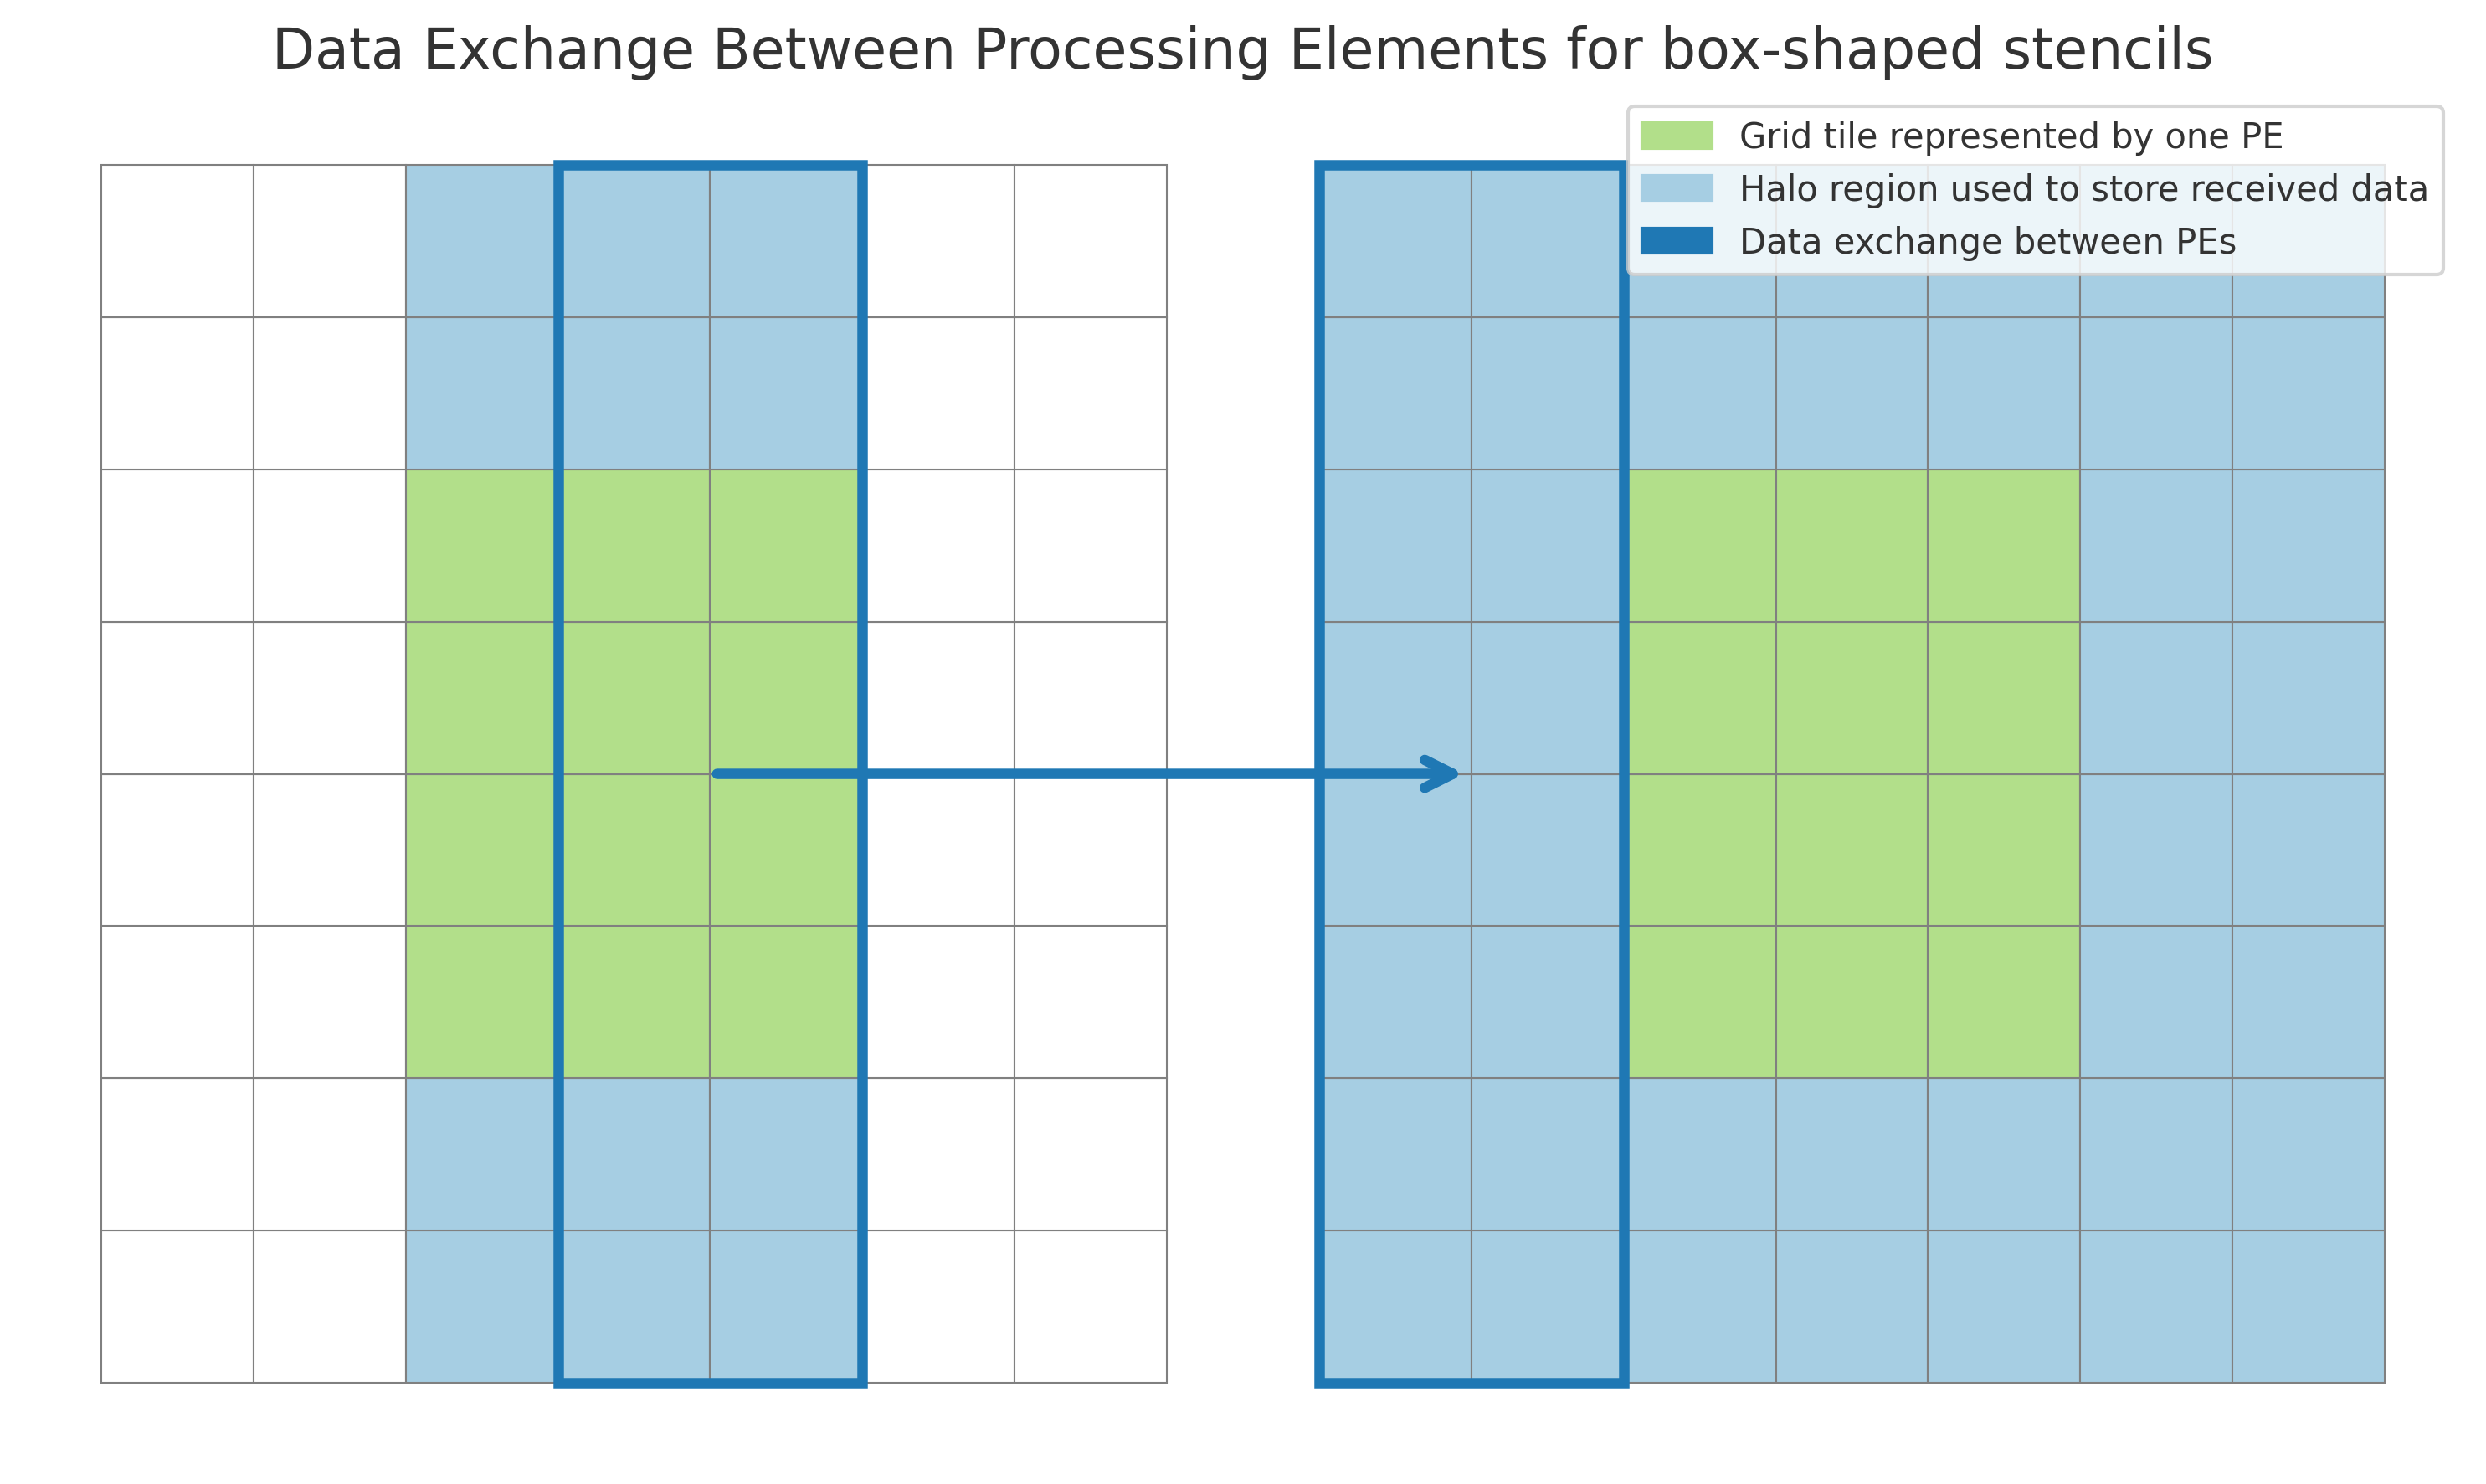
\includegraphics[width=0.7\textwidth]{box_shaped_data_exchange.png}
    \caption{Data exchange pattern between neighboring PEs for box-shaped stencil implementation showing sequential communication steps}
    \label{fig:data_exchange_box_shaped}
\end{figure}

Although multi-hop communication could be implemented to allow a large radius while using a small tile size, the benefit would likely not justify the additional complexity in the routing logic and the additional communication steps. Using larger tile sizes, which we found in general to be more efficient, so multi-hop communication isn't required even for high-order stencils.

The Neumann boundary condition uses information about the derivative of the solution at the border regions to improve the solution for certain stencils, and could also be an interesting extension. A periodic boundary condition would present a major challenge on the \ac{wse} as it would involve communication of \acp{pe} with a high spatial distance. 

Similar to the research done for other \ac{hpc} architectures, we expect automated code generation tools or compiler pipelines targeting the \ac{wse}, to become more important.
Existing approaches for 3D stencils\cite{sai2024automated} could be extended to also support optimized solutions for 2D stencils and automatically choosing parameters to result in highest throughput kernels.
Integrating these approaches into existing stencil \acp{dsl} to support the \ac{wse} as one of multiple possible backends would be a valuable contribution to make the \ac{wse} a more versatile tool for stencil computations.